\chapter{Test on Simulation of Miniature Racing Vehicle}\label{chap:test-chronos}

In this chapter, we present the test of the safety filter introduced in \cref{chap:robust-ddsf-lti}, the prediction method and dataset evaluation metric introduced in \cref{chap:non-linear-system} on the simulation of a miniature racing vehicle.
We will first introduce the vehicle model and simulation setup, including the simplified kinematic model and the more realistic dynamic model.
We also discuss the design and choice of terminal ingredient for this model, and briefly discuss how can we evaluate the performance of the safety filter.
Then the result for kinematic model will be presented, showing that for this simple non-linear model, the indirect formulation of robust safety filter introduced in \cref{sec:indirect-formulation} can successfully guarantee safety, even when the output is noisy.
Finally, we present the result for the dynamic model, showing that the robust safety filter equipped with prediction method introduced in \cref{sec:weighting-method} can also guarantee safety for this more realistic model, when we have access to the noise-free output, proper hyperparameters, and rich enough dataset.


\section{Vehicle Model and Simulation Setup}\label{sec:model-sim-setup}

In this section, we introduce the vehicle model and simulation setup used in this chapter.
Our model is based on the RC racing vehicle \emph{Chronos}, and its simulation/control framework \emph{CRS} as introduced in \cite{carronChronosCRSDesign2022}.

\subsection{Vehicle Model}\label{subsec:vehicle-model}

We have two different models for the vehicle, the kinematic model and the more realistic dynamic model, as introduced in \cite{carronChronosCRSDesign2022}.
They are both based on world-frame coordinates, independent of track on which the vehicle is running.
% For example, the model is successfully used for the design of the safety filter in \cite{tearlePredictiveSafetyFilterRacing2021}.

However, for the data-driven predictive safety filter, we need to find an equilibrium of the system, and the system will be operating around this equilibrium.
This model based on world-frame does not guarantee such a good equilibrium.
In contrast, the track-relative coordinates introduced in \cite{tearlePredictiveSafetyFilterRacing2021} is more suitable for the data-driven predictive safety filter.
We can also design different equilibrium for track-relative coordinates, as will be introduced in \cref{sec:result-kinematic-model}.

As can be seen in \cref{fig:track-relative-coordinates}, the track-relative coordinates are defined for a certain piece of track, with $\elat$ being the deviation of vehicle from the centerline, and $\mu$ being the difference of heading angle from the tangent of the centerline, $l$ being the progress of vehicle along the centerline.

\includefig{error-dynamics.pdf}{0.5}{Track-relative coordinates.}{fig:track-relative-coordinates}

The kinematic model in track-relative coordinates can be written in \cref{eq:kinematic-model}, as modified from \cite{tearlePredictiveSafetyFilterRacing2021}.
\begin{subequations}
\label{eq:kinematic-model}
\begin{gather}
    x = \begin{bmatrix}
        \elat \\
        \mu \\
        v \\
        l
    \end{bmatrix} 
    , \; u = \begin{bmatrix}
        \tau \\
        \delta
    \end{bmatrix} \textperiod \label{eq:kinematic-state} \\
    \dot{x} = \begin{bmatrix}
        v \sin\left(\mu + \beta\right) \\
        \frac{v}{l_r} \sin\left(\beta\right) - c \frac{v \cos\left(\mu + \beta\right)}{1 - c \elat} \\
        \frac{\tau}{m} \\
        \frac{v \cos\left(\mu + \beta\right)}{1 - c \elat}
    \end{bmatrix}, \; 
    \beta = \atangent\left(\frac{l_r}{l_r + l_f} \tan(\delta)\right) \textperiod \label{eq:kinematic-dynamics}
\end{gather}
\end{subequations}
where $x$ is the state, $u$ is the input, $m$, $l_f$ and $l_r$ are the mass, distance from the vehicle to front and rear axes, respectively, $c$ is the curvature of the track.
We assume we can observe the output:
\begin{equation}\label{eq:kinematic-output}
    y = \transpose{\begin{bmatrix}\elat & \mu & v\end{bmatrix}} \textstop
\end{equation}

And the dynamic model in track-relative coordinates can be written in \cref{eq:dynamic-model}, as introduced in \cite{carronChronosCRSDesign2022,tearlePredictiveSafetyFilterRacing2021}.
\begin{subequations}
    \label{eq:dynamic-model}
    \begin{gather}
        x = \begin{bmatrix}
            \elat \\
            \mu \\
            \vx \\
            \vy \\
            r \\
            l
        \end{bmatrix} 
        , \; u = \begin{bmatrix}
            \tau \\
            \delta
        \end{bmatrix} \textperiod \label{eq:dynamic-state} \\
        \dot{x} = \begin{bmatrix}
            \vx \sin(\mu) + \vy \cos(\mu) \\
            r - c \frac{\vx \cos(\mu) - \vy \sin(\mu)}{1 - c \elat} \\
            \frac{1}{m} \left(F_x - F_f \sin(\delta) + m \vy r\right) \\
            \frac{1}{m} \left(F_r + F_f \cos(\delta) - m \vx r\right) \\
            \frac{1}{I_z} \left(F_f l_f \cos(\delta) - F_r l_r\right) \\
            \frac{\vx \cos(\mu) - \vy \sin(\mu)}{1 - c \elat}
        \end{bmatrix} \textperiod \label{eq:dynamic-dynamics}
    \end{gather}
\end{subequations}
where $I_z$ is the moment of inertia, $r$ is the yaw rate, $F_x$, $F_f$ and $F_r$ are the longitudinal force, front lateral force and rear lateral force, as introduced by the tire model:
\begin{subequations}
    \label{eq:tire-model}
    \begin{gather}
        \alpha_f = \atangent\left(\frac{\vy + l_f r}{\vx}\right) - \delta \textperiod \; 
        \alpha_r = \atangent\left(\frac{\vy - l_r r}{\vx}\right) \textperiod \label{eq:tire-slip-angle} \\
        F_{f/r} = D_{f/r} \sin\left(C_{f/r} \atangent\left(B_{f/r} \alpha_{f/r}\right)\right) \textperiod \label{eq:tire-lateral-force} \\
        F_x = \left(C_{m1} - C_{m2} \vx\right) \tau - C_d \vx^2 - C_{\text{roll}} \textperiod \label{eq:tire-longitudinal-force}
    \end{gather}
\end{subequations}
where $D_{f/r}$, $C_{f/r}$, $B_{f/r}$, $C_{m1}$, $C_{m2}$, $C_d$ and $C_{\text{roll}}$ are the tire parameters.
We assume we can observe the output:
\begin{equation}\label{eq:dynamic-output}
    y = \transpose{\begin{bmatrix}\elat & \mu & \vx & \vy\end{bmatrix}} \textstop
\end{equation}

\subsection{Simulation Setup}\label{subsec:simulation-setup}

In general, the can have a varying curvature and width.
For simplicity, we only work with track of width $w=\SI{0.5}{m}$ with piece wise constant curvature.
As can be seen from \cref{eq:kinematic-model,eq:dynamic-model}, the curvature $c$ is a parameter of the model, so it is necessary to change the model when the curvature changes.
To simplify the problem, we only use a fixed curvature and a fixed model when solving the optimization problem \cref{eq:robust-ddsf-indirect}.
In each time step, we choose the curvature and corresponding model according to current position of the vehicle on the track heuristically, by looking ahead a certain distance in the progress on track center $l$.

In practice, the constraint \emph{the vehicle should not hit the track boundary} can be complicated to formulate, considering the vehicle shape \cite{tearlePredictiveSafetyFilterRacing2021}.
Within this chapter, to simplify the problem, we view the vehicle as a point of mass, and the constraint is simplified to $-\frac{w}{2} \leq \elat \leq \frac{w}{2}$.
We also impose a constraint on the heading angle $\mu$: $-\frac{\pi}{2} \leq \mu \leq \frac{\pi}{2}$, to avoid the vehicle from driving backwards.

To avoid the complexity of real leaning-based controllers, open-loop unsafe control inputs are used as objective inputs.

We use a numerical ode solver CVODE \cite{gardner2022sundials} via the CasADi \cite{AnderssonCasadi2019} interface to simulate the vehicle, and discretize the model \cref{eq:kinematic-model,eq:dynamic-model} with sampling time $\SI{0.01}{s}$.
The optimization problem \cref{eq:robust-ddsf-indirect} is solved by MOSEK \cite{mosek}.
% For the kinematic model, we set the output of system to $\transpose{\begin{bmatrix}\elat & \mu & v\end{bmatrix}}$, for the dynamic model, it will be $\transpose{\begin{bmatrix}\elat & \mu & \vx & \vy\end{bmatrix}}$.
More specific setups, including other parameters, constraints, initial conditions, hyperparameters for the safety filter, and scheme for choosing leaning based inputs, will be introduced in the corresponding sections.


\section{Design of Terminal Ingredient}\label{sec:design-terminal-ingredient}

Before we present the result for the safety filter, we need to discuss the design and choice of terminal ingredient for the vehicle model.
Note that, although this design process takes usage of \emph{formualtion} the vehicle dynamics \cref{eq:kinematic-model} and \cref{eq:dynamic-model}, it does not require any knowledge of the \emph{parameters} of the vehicle dynamics.

Within the scope of this thesis, we set the terminal constraint to an equilibrium of the system, so the question is reduced to finding an equilibrium of the system.

By investigating the vehicle model \cref{eq:kinematic-model,eq:dynamic-model}, we can propose the following schemes to find an equilibrium.
Note that they are designed for a constant curvature, since we only use a fixed curvature and a fixed model when solving the optimization problem \cref{eq:robust-ddsf-indirect}, as mentioned in \cref{subsec:simulation-setup}.

\paragraph{Fitting an Equilibrium with Constant $\elat$ and $v$}
Considering the kinematic model \cref{eq:kinematic-model}, for certain deviation from centerline $\elat$ and velocity $v$, we can find a constant heading angle $\mu$ and steering angle $\delta$ that will keep $\elat$ and $v$ constant, with zero acceleration $\tau = 0$.
This corresponds to the case where the vehicle is steering with constant radius $1/c - \elat$ and constant velocity $v$.
However, without further knowledge about the system parameters, it is hard to find the value of $\mu$ and $\delta$ corresponding to a given $\elat$ and $v$.
We can use the dataset and \cref{lemma:fundamental-lemma} to fit for the value of $\mu$ and $\us$ corresponding to a given $\elat$ and $v$, by the fact that if we set the system into equilibrium, the output will not change over time:
\begin{equation}\label{eq:fitting-equilibrium}
    \vRepeatVec{\ys}{L} = \Yf \pinv{\hankeluyone} \begin{bmatrix}
        \vRepeatVec{\us}{l} \\
        \vRepeatVec{\us}{L} \\
        \vRepeatVec{\ys}{l} \\
        1
    \end{bmatrix} \textperiod
\end{equation}
where we require the predicted output sequence $\vRepeatVec{\ys}{L}$ to be the equilibrium $\ys$, under the extended initial condition $\begin{bmatrix}\vRepeatVec{\us}{l} & \vRepeatVec{\ys}{l}\end{bmatrix}$ and proposed inputs $\vRepeatVec{\us}{L}$.
By fixing $\elat$ and $v$ in $\ys$, we can infer a linear system from \cref{eq:fitting-equilibrium} and solve it for $\mu$ and $\delta$.

\paragraph{Fixing $\mu$ and Velocity in Optimization Problem}
Another observation is, if the heading angle $\mu$ and velocity $v$ are fixed, an equilibrium is also implicitly defined.
% This holds for both the kinematic model \cref{eq:kinematic-model} and the dynamic model \cref{eq:dynamic-model}.
Although it is also possible to fit other variables similarly in \cref{eq:fitting-equilibrium}, here we choose another method to find the equilibrium.
Similar to the method in \cite{mullerDataDrivenQCR2022}, where the equilibrium is implicitly defined and decided by the predictor, we can also let the dynamic constraint \cref{eq:robust-ddsf-indirect-dynamic} and terminal constraint \cref{eq:robust-ddsf-indirect-terminal} decide the equilibrium.
In the terminal constraint, the velocity is constrained to be a certain constant $v_0$.
The heading angle $\mu$, deviation from centerline $\elat$, and steering angle $\delta$ is constrained to be the same for the last $n$ time steps, but the specific values are not constrained.

\paragraph{Stopping at a Certain Point}
Another choice of equilibrium for the vehicle is to stop it at a certain point.
% We can choose to stop the vehicle at a certain point, for example on the centerline, or let it stop anywhere on the track.
As for the constraint, we can constrain the velocity to be zero for the last $n$ steps.
Other variables can be constrained to be the same for the last $n$ steps, or be set to specific values for the last $n$ steps.
For example, we can constrain the deviation from centerline $\elat$ to be zero, and the heading angle $\mu$ to be zero, so the vehicle will stop on the centerline with zero heading angle.

We implemented all the methods mentioned above to the kinematic model, with some model-specific design add (for example in some cases we can fix the throttle $\tau_s = 0$).
And the results are presented and discussed in \cref{sec:result-kinematic-model}.
For the dynamic model, we only use the ``Fixing $\mu$ and Velocity in Optimization Problem'' method, and the result is presented and discussed in \cref{sec:result-dynamic-model}.


\section{Simulation Using Kinematic Model}\label{sec:result-kinematic-model}

In this section, we present the result for the safety filter on the kinematic model.
For the dataset and online observation, we set the noise level to $\SI{1}{\milli\meter}$ for position on both $x$ and $y$ axis, $\SI{0.01}{\radian}$ for heading angle, and $\SI{0.005}{\meter/\second}$ for $v$.
Each noise is sampled from a uniform distribution with the given range.
Here we present the result with unsafe open-loop objective input consisting of sine wave acceleration and steering input.
The terminal ingredient is chosen to be the ``Fixing $\mu$ and Velocity in Optimization Problem'' method.
For the hyperparameters in \cref{eq:robust-ddsf-direct}, we choose prediction horizon of $L = 150$, corresponding to $\SI{1.5}{\second}$.
The number of input-output pairs used for initial condition is set to $l = 15$.
The constraint tightening constants are set to:
\begin{align*}
    [c_1, c_2, c_3, c_{i \geq 4}] &= [0.25, 0.1, 0.05, 0.01] \times w/2 \text{ for } \elat \textperiod \\
    [c_1, c_2, c_3, c_{i \geq 4}] &= [0.1, 0.1, 0.05, 0.01] \times 0.5 \pi \text{ for } \mu \textstop
\end{align*}
% $[0.25, 0.1, 0.05, 0.01] \times w/2$ for $\elat$ and $[0.1, 0.1, 0.05, 0.01] \times 0.5 \pi$ for $\mu$.
Regularization parameter $\lamsigma$ is set to $50000$.

We use a dataset of length $N = 1000$ for each curvature.
The dataset is collected by simulating the system for $1000$ time steps, starting from the equilibrium of system $\ys$, and applying a random input added by the equilibrium input $\us$.
The equilibrium $\us$ and $\ys$ is found by solving a non-linear equation using system dynamics \cref{eq:kinematic-model}, fixing $\elat=0$ and $v=\SI{1}{\meter/\second}$.
This dataset collection process designed to collect a dataset close to the designed equilibrium, but is not realistic, since it uses knowledge of the system parameters.
In practice, we can use manual input to keep the system around the equilibrium when collecting the dataset, or use a more realistic data-collection scheme as introduced in \cref{fig:data-collection-process}.

\begin{figure}[ht]
    \centering
    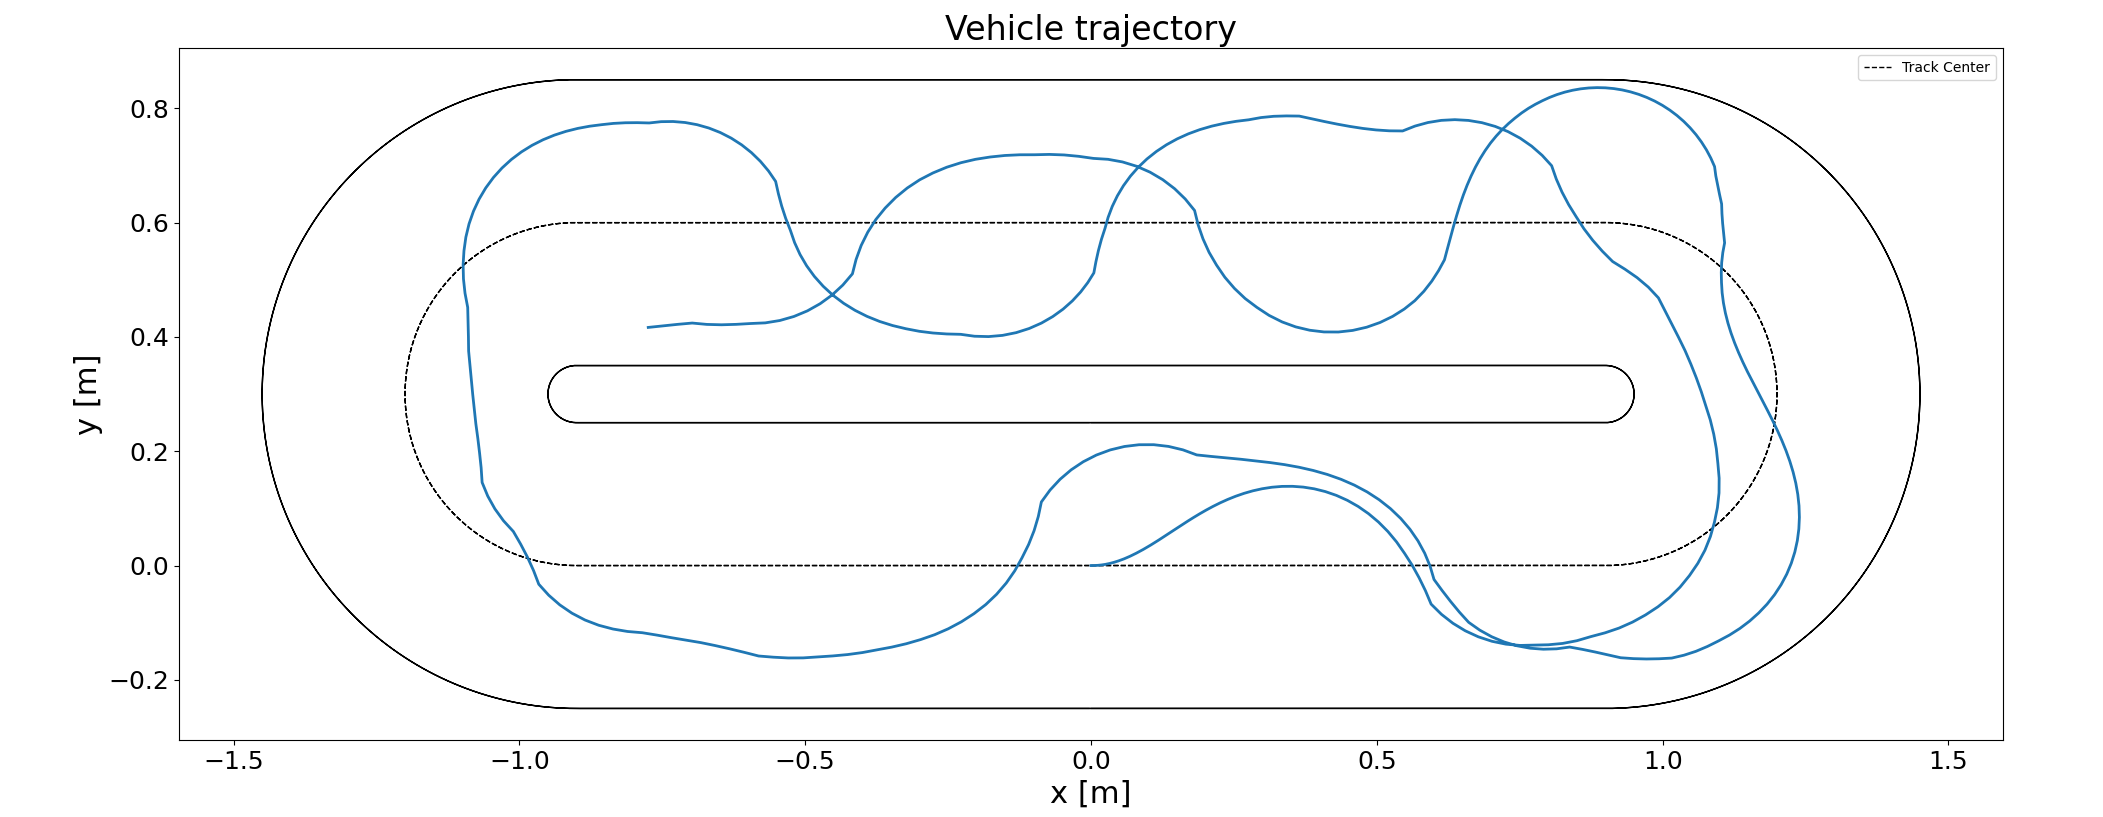
\includegraphics[width=0.9\textwidth]{\imagedir/kinematic-trajectory.png}
    \caption{Path of the vehicle, the dotted line being the track centerline and the blue line being the path.}
    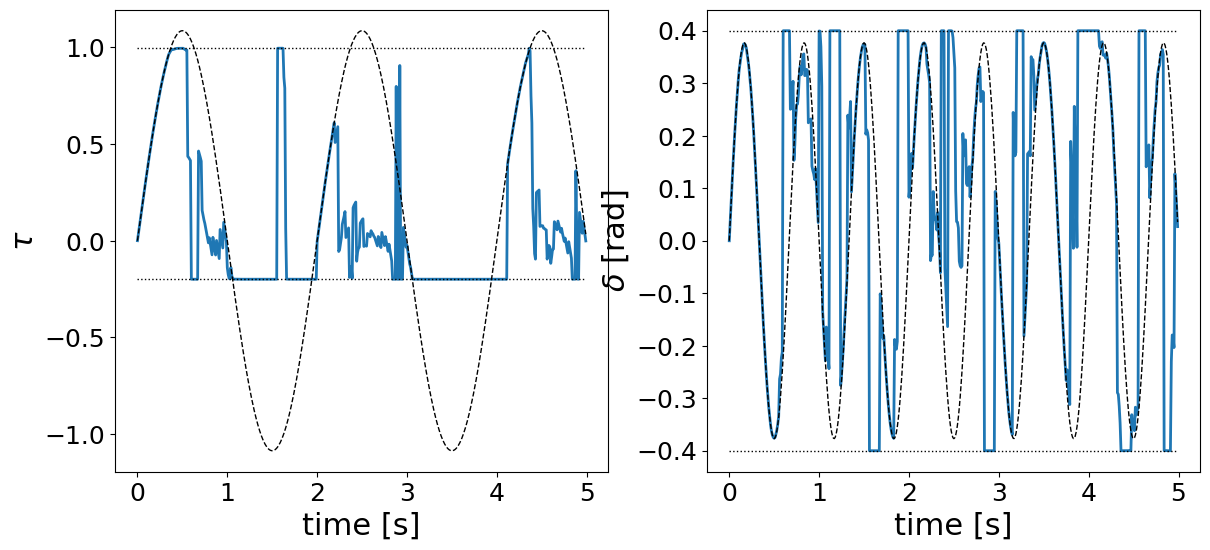
\includegraphics[width=0.9\textwidth]{\imagedir/kinematic-sin-sin-inputs.png}
    \caption{Objective and applied inputs, the dotted line being the unsafe open-loop objective input and blue line being the applied input.}
    \label{fig:kinematic-single-run}
\end{figure}

We can see from \cref{fig:kinematic-single-run}, the objective inputs are modified by the safety filter and it successfully keeps the vehicle on the track.

We also present the result of applying different terminal ingredients, as mentioned in \cref{sec:design-terminal-ingredient}.
Here the unsafe open-loop objective input is set to full throttle $\tau_s = \tau_{\max}$.
The hyperparameters including the prediction horizon, and constraint tightenings, are adjusted for each terminal ingredient.
To avoid the hyperparameters to overfit to this specific objective control, they are tuned so to make sure that the vehicle can successfully drive around the track with three different objective control input rules, including `Max Throttle with Zero Steering', `Max Throttle with Sine Steering' and `Sine Throttle with Sine Steering'.

\begin{figure}[ht]
    \centering
    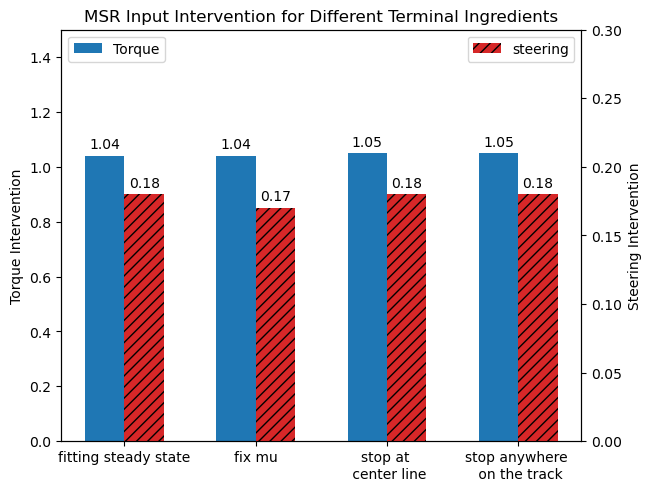
\includegraphics[width=0.7\textwidth]{\imagedir/kinematic-terminal-comparison.png}
    \caption{Input interference for different terminal ingredients.}
    \label{fig:kinematic-terminal-comparison}
\end{figure}

We can see from \cref{fig:kinematic-terminal-comparison} that, with finely tuned hyperparameters, all the terminal ingredients have very similar mean squared input interference.
It may reflect that, with the hyperparameters being tuned accordingly, the performance of the safety filter is not sensitive to the choice of terminal ingredient for this setup.

It's worth noting that, it's not necessary true that smaller mean squared input interference means better performance for a safety filter.
For example, a safety filter can have smaller mean squared input interference by always modifying the input to some point, so the vehicle can always stay near the centerline.
While another safety filter will only make large interference when the vehicle is about to leave the track, resulting in a larger mean square input interference.
However, the second safety filter is more desirable, as it will not interfere with the vehicle when it is driving normally.
% There are no good metrics to evaluate the performance of a safety filter yet, and we will not discuss this topic further in this Thesis.
It's difficult to evaluate the performance of safety filters with a single metric, as for different applications and different scenarios, we may care about different aspects of the safety filter.
For example, for a safety filter designed for autonomous racing, we may want to minimize lap time under the full acceleration unsafe objective input; while for a safety filter designed for a specific learning-based controller, we may want to minimize the input interference at the end of training process.
Further discussion on this topic is out of the scope of this thesis.


\newpage
\section{Simulation Using Dynamic Model}\label{sec:result-dynamic-model}

This section presents the result for the safety filter on the dynamic model.
We only use the ``Fixing $\mu$ and Velocity in Optimization Problem'' method to find the terminal ingredient.

Also, we assume we have noise-free access to the output, both in the dataset and online observation.
We take use of the prediction method introduced in \cref{chap:non-linear-system} to make predictions for the dynamic model, and use the formulation \cref{eq:robust-ddsf-weighting} as the safety filter.
The optimization problem \cref{eq:robust-ddsf-indirect} is also solved by MOSEK \cite{mosek}.
The prediction horizon is set to $L=80$, number of input-output pairs used for initial condition set to $l=10$, and the constraint tightening constants being:
\begin{align*}
    [c_1, c_2, c_3, c_{i \geq 4}] &= [0.25, 0.1, 0.05, 0.01] \times \elat_{\max} \text{ for } \elat \textperiod \\
    [c_1, c_2, c_3, c_{i \geq 4}] &= [0.2, 0.1, 0.05, 0.01] \times \mu_{\max} \text{ for } \mu \textperiod \\
    [c_1, c_2, c_3, c_{i \geq 4}] &= [0.2, 0.1, 0.05, 0.01] \times \vx_{\max} \text{ for } \vx \textperiod \\
    [c_1, c_2, c_3, c_{i \geq 4}] &= [0.1, 0.05, 0.01, 0.005] \times \vy_{\max} \text{ for } \vy \textstop
\end{align*}
For the prediction method, we choose diagonal $Q$, where each $Q_{ii}$ is the reciprocal of the range of corresponding element in the extended state, so that all the input/outputs are normalized by the corresponding maximum value, and the weighting function $w(d) = \frac{1}{d}$.
Similar to the case in \cref{sec:non-linear-system-numerical-example}, we only use the trajectory slices that are close enough to current initial state, if enough number of such slices are available.

We introduce a scheme of collecting more dataset with a more realistic method, as can be seen in \cref{fig:data-collection-process}.
This scheme is similar to the \emph{DAgger} algorithm in \cite{rossReductionImitationLearning2011}, where the policy is updated and new dataset using the new policy is added to the existing dataset at each iteration.
In our scheme, we do not use dataset to train a policy, but directly use it for the safety filter.
The scheme starts with a dataset collected offline, and enters the application phase first.
In the application phase, the system is equipped with the safety filter with current dataset, and several runs with different learning-based controllers or unsafe open-loop objective inputs are performed.
If the safety filter is able to keep the system safe for all the runs, the scheme stops.
Otherwise, the dataset collection phase starts, where the system is equipped with the safety filter with current dataset, and an exploring controller or rich enough unsafe open-loop objective input is used to collect more dataset.
After this dataset collection phase, the new dataset is added to the existing dataset, and the application phase starts again.

\includefig{data-collection-process.pdf}{0.9}{The process of dataset collection, each run uses a different controller or objective input scheme, and stops after safe constraint not satisfied.}{fig:data-collection-process}

For our simulation, a dataset trajectory of length $N=1000$ is collected, by a similar method in \cref{sec:result-kinematic-model}, as the offline dataset.
We use random inputs as objective inputs in the dataset collection process; and apply three different kinds of open loop objective inputs in the application runs, as introduced in \cref{sec:result-kinematic-model}.

As the final result, at the sixth application phase, the safety filter is able to keep the vehicle within the track boundaries for all three types of unsafe open-loop objective inputs.
Here we present the trajectory and inputs with the objective input being `Sine Throttle with Sine Steering', as can be seen in \cref{fig:dynamic-single-run}.

\begin{figure}[ht]
    \centering
    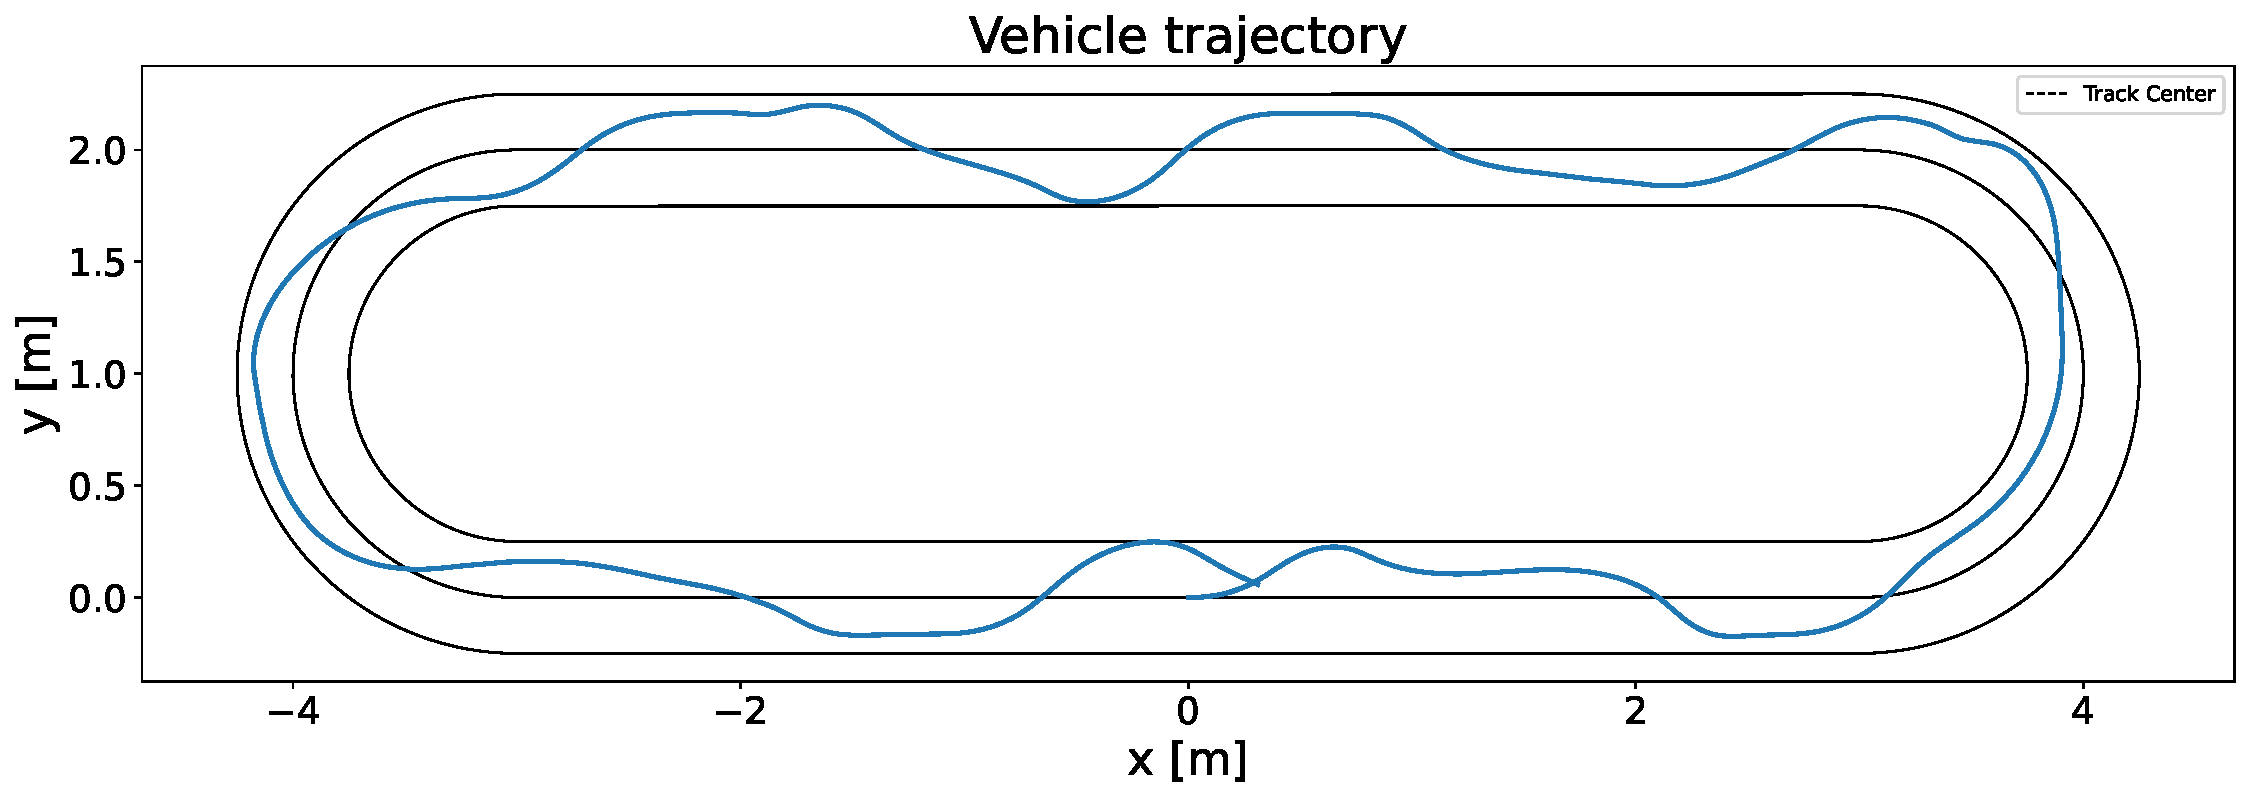
\includegraphics[width=0.9\textwidth]{\imagedir/dynamic-simulation-single-trajectory.pdf}
    \caption{Path of the vehicle, the dotted line being the track centerline and the blue line being the path.}
    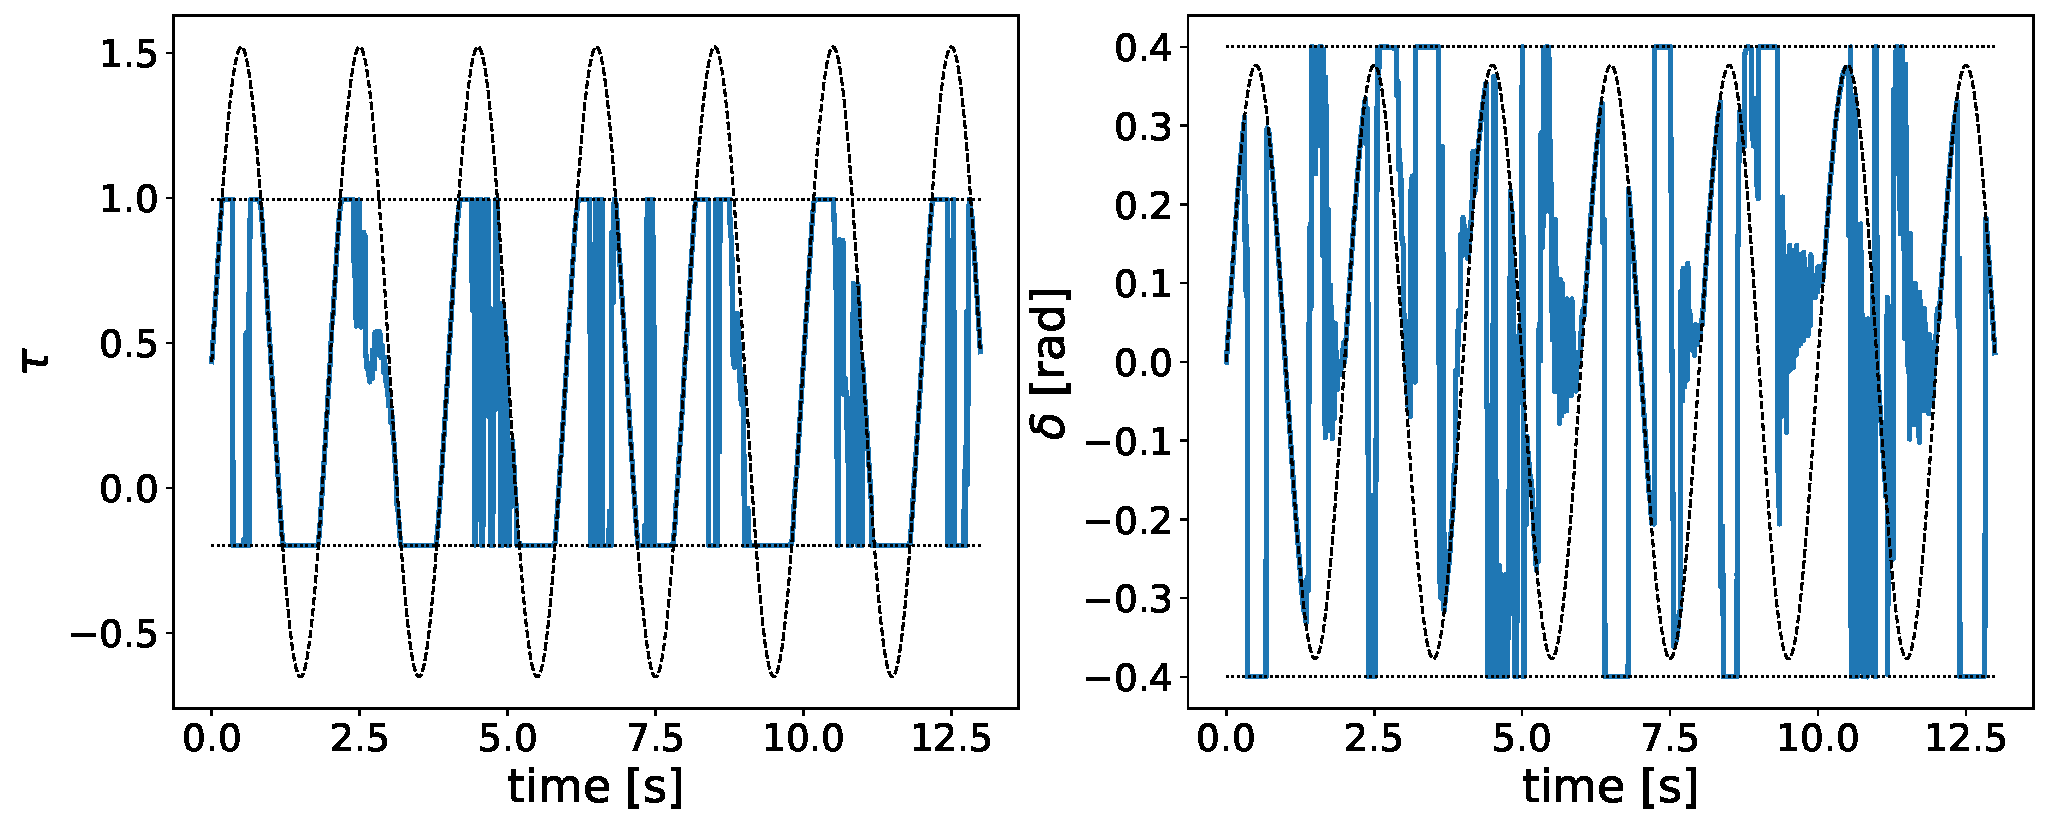
\includegraphics[width=0.9\textwidth]{\imagedir/dynamic-simulation-inputs.pdf}
    \caption{Objective and applied inputs, the dotted line being the unsafe open-loop objective input and blue line being the applied input.}
    \label{fig:dynamic-single-run}
\end{figure}

We can see from \cref{fig:dynamic-single-run}, the safety filter is able to keep the vehicle within the track boundaries, even with the more realistic dynamic model.

We also compare the six datasets used in application phases, by the metric introduced in \cref{sec:fractal-dimension-method}.
The input-output space in this case is $\RealVec{m+p} = \RealVec{6}$, but as mentioned in \cref{sec:fractal-dimension-method}, due to computational complexity, we only use the output part in $\RealVec{p} = \RealVec{4}$.
As can be seen from \cref{fig:box-counting-dimension-dynamic-test}, the dataset becomes more and more rich for later application phases, as more data is added in the dataset collection phase.

\includefig{box-counting-dimension-dynamic-test.pdf}{0.7}{Comparing six datasets used in application phases, $\dataset_0$ to $\dataset_5$ correspond to the dataset used in the first to sixth phase, respectively.}{fig:box-counting-dimension-dynamic-test}

There are still many improvements to be made for the safety filter, though.
For example, the resulting input sequence is not smooth, and can not be applied to the real RC vehicle.
Also, similar improvements mentioned for the prediction method in \cref{sec:weighting-method} can also be applied to the safety filter.
These possibilities are left for future work.
